\documentclass[12pt]{exam}
\usepackage[utf8]{inputenc}

\usepackage[margin=1in]{geometry}
\usepackage{amsmath,amssymb}
\usepackage{multicol}
\usepackage{mathrsfs}
\usepackage{amsmath}
\usepackage{graphicx}
\usepackage{tikz}
\usepackage{forest}
\tikzset{
  tree node/.style = {align=center, inner sep=0pt, font = \scriptsize},
  S/.style = {draw, circle, minimum size = 8mm, top color=white, bottom color=black!20},
  tree node label/.style={font=\scriptsize},
}
\forestset{
  declare toks={left branch prefix}{},
  declare toks={right branch prefix}{},
  declare toks={left branch suffix}{},
  declare toks={right branch suffix}{},
  tree node left label/.style={
    label=180:#1,
  },
  tree node right label/.style={
    label=0:#1,
  },
  maths branch labels/.style={
    branch label/.style={
      if n=1{
        edge label={node [left, midway] {$\forestoption{left branch prefix}##1\forestoption{left branch suffix}$}},
      }{
        edge label={node [right, midway] {$\forestoption{right branch prefix}##1\forestoption{right branch suffix}$}},
      }
    },
  },
  text branch labels/.style={
    branch label/.style={
      if n=1{
        edge label={node [left, midway] {\foresteoption{left branch prefix}##1\forestoption{left branch suffix}}},
      }{
        edge label={node [right, midway] {\forestoption{right branch prefix}##1\forestoption{right branch suffix}}},
      }
    },
  },
  text branch labels,
  set branch labels/.style n args=4{%
    left branch prefix={#1},
    left branch suffix={#2},
    right branch prefix={#3},
    right branch suffix={#4},
  },
  set maths branch labels/.style n args=4{
    maths branch labels,
    set branch labels={#1}{#2}{#3}{#4},
  },
  set text branch labels/.style n args=4{
    text branch labels,
    set branch labels={#1}{#2}{#3}{#4},
  },
  branch and bound/.style={
    /tikz/every label/.append style=tree node label,
    maths branch labels,
    for tree={
      tree node,
      S,
      math content,
      s sep'+=30mm,
      l sep'+=15mm,
      thick,
      edge+={thick},
    },
    before typesetting nodes={
      for tree={
        split option={content}{:}{tree node left label,content,tree node right label,branch label},
      },
    },
    where n children=0{
      tikz+={
        \draw [thick]  ([yshift=-10pt, xshift=-2.5pt].south west) -- ([yshift=-10pt, xshift=2.5pt].south east);
      }
    }{},
  },
}
\usepackage{tikz-qtree}
\usetikzlibrary{calc, shapes}

\newcommand{\class}{SA 405}
\newcommand{\term}{Fall 2018}
\newcommand{\examnum}{Final Exam}
\newcommand{\examdate}{Dec 14, 2018}
\newcommand{\timelimit}{180 Minutes}

\pagestyle{head}
\firstpageheader{}{}{}
\runningheader{\class}{\examnum\ - Page \thepage\ of \numpages}{\examdate}
\runningheadrule

%% Answer box macros
%% \answerbox{alignment}{width}{height}
\newcommand{\answerbox}[3]{%
  \fbox{%
    \begin{minipage}[#1]{#2}
      \hfill\vspace{#3}
    \end{minipage}
  }
}

%% \answerboxfull{alignment}{height}
\newcommand{\answerboxfull}[2]{%
  \answerbox{#1}{6.38in}{#2} 
}

%% \answerboxone{alignment}{height} -- for first-level bullet
\newcommand{\answerboxone}[2]{%
  \answerbox{#1}{6.0in}{#2} 
}

%% special boxes
\newcommand{\wordbox}{\answerbox{c}{1.2in}{.7cm}}
\newcommand{\catbox}{\answerbox{c}{.5in}{.7cm}}
\newcommand{\letterbox}{\answerbox{c}{.7cm}{.7cm}}



\begin{document}

\noindent
\begin{tabular*}{\textwidth}{l @{\extracolsep{\fill}} r @{\extracolsep{6pt}} r}
\textbf{\class} &&\textbf{\examnum}\\
\textbf{\term} &&\textbf{\examdate}\\
 && \\
 && \\
Midshipmen are persons of integrity.& \textbf{Name:} & \makebox[2.2in]{\hrulefill}\\\\
%\textbf{Time Limit: \timelimit} & Teaching Assistant & \makebox[2in]{\hrulefill}
\end{tabular*}

\noindent
\rule[2ex]{\textwidth}{2pt}

%This exam contains \numpages\ pages (including this cover page) and \numquestions\ questions.\\
%Total of points is \numpoints.

\begin{itemize}
\item Do {\bf not} write your name on each page, only write your name above.

\item No books or notes % or calculators
% that do symbolic manipulation (such as TI-89 or TI-92) 
 are allowed. %{\bf One} 8.5 by 11 inch formula/note sheet is allowed.

%\item You may use your calculator on this test.

\item Show all work clearly. (Little or no credit will be given for a numerical
answer without the correct accompanying work.
Partial credit is given where appropriate.) 

%\item If you need more space than is provided, use the back of the previous page. 

\item Please read the question carefully.
If you are not sure what a question is
asking, ask for clarification.

\item If you start over on a problem, please CLEARLY indicate what your final
  answer is, along with its accompanying work.

\item All formulations must have descriptions of any indices, parameters, and decision variables used. All constraints must be described. 
\end{itemize}


\begin{center}
Grade Table (for teacher use only)\\
\addpoints
\gradetable[v][questions]
\end{center}

\noindent
\rule[2ex]{\textwidth}{2pt}

\newpage %%%%%%%





All possible modeling topics
\begin{itemize}

	\item Network flow problems

	\begin{itemize}

		\item Shortest path problem
 
 The Superintendent asks his most trusted Ops Research majors (you all) to give him directions from the Yard to Los Angeles, CA. Of course, he wants to find the path the minimizes his total travel time. Assume that he can travel through a set of cities $\mathcal{C}$ along a set of roads $\mathcal{A}$ between each city. He assumes that traveling along some arc $(i,j) \in \mathcal{A}$ will require $t_{ij} > 0$ minutes.  


\begin{parts}

\part Define your starting node $s$ and your destination/termination node $t$. Using these definitions, formulate an abstract mathematical programming model to help the superintendent solve his problem.

%\vspace{11cm}

\part The superintendent now wants to consider traffic delays in each city. To account for this added time it takes to travel through each city, he assumes that it will take $d_i > 0$ extra units of time to travel through city $i \in \mathcal{C}$. Identify and define any additional variables and/or constrains, and modify your mathematical programming model above to account for the extra traffic-related time delays.
\end{parts}

		\item Maximum Flow
\\
Ad-hoc networks are made up of low-powered wireless devices. These networks can be used on battlefields, in regions that have recently suffered from natural disasters, and in other hard-to-reach areas. The idea is that a large collection of cheap, simple devices could be distributed through the area of interest (for example, by dropping them from an airplane); the devices would then automatically configure themselves into a functioning wireless network. These devices are used to gather as much information about a network as possible. Define your destination/collection node $t$ where all gathered information is to be analyzed. Additionally, these networks adhere to multi-hop communication, in which each device can relay information originating at another node along to the sink $t$.

Definitions:
\begin{itemize}
	\item Set $\mathcal{V}$ of devices.
	\item Set $\mathcal{A}$ of connections $(i,j) \mathcal{A}$ between devices $i, \ j \in \mathcal{V}$.
	\item Maximum amount of information that can be sent on connection $(i,j) \in \mathcal{A}$ is $c_{ij}$.

\end{itemize}

\begin{parts}
\part  Formulate an abstract mathematical programming model to maximize the total amount of information gathered by all devices. \emph{Hint:} Consider adding \emph{dummy} node(s).

\end{parts}

	\end{itemize}

	\item Fixed-charge problem
	\begin{itemize}
		\item weak-forcing
		\item strong-forcing

		I feel like my mids have been tested over this pretty thoroughly.
	\end{itemize}

	\item Set-covering, packing, and partitioning constraints----I think that we can test them over these on the facility location problem.

	\item Logical Constraints
	\begin{itemize}
		\item These can be added throughout as subproblems.
	\end{itemize}
	
	\item Minimum Spanning Tree
	\begin{itemize}
		\item They've been tested over this and had a quiz. Maybe we could just ask them to identify a problem of this type and run Prims?
	\end{itemize}
	\item Travelling salesperson problem
	\begin{itemize}
		\item I say we go with a vehicle routing problem here? What do you think?
	\end{itemize}
	\item Vehicle Routing problem


Your regional manager, Michael Scott, has asked you to solve a Vehicle Routing Problem (VRP) to determine an optimal set of 3 paper-delivery routes that begin and end at their warehouse in Scranton, PA. At least one of these routes must visit each one of the 12 customers found in the Paper Belt. Each vehicle must be used and can transport no more than 250 cases of paper, and must visit at least two customers. He also tells you that his goal is to minimize the total distance traveled among all vehicles. 



\vspace{.5cm}
Answer the following questions related to Michael Scott's request.
\begin{parts}
\item Please provide the \textbf{concrete} integer programming model for solving Mr. Scott's problem above. Clearly define your objective function, constraints, and any variables and parameters required.
\item You solve the problem, and your solution contains a cycle of customers $1, 4, and 5$. Please provide the appropriate set of subtour-elimination constraints.\\
\answerboxone{c}{1.5in}
\item You solve the problem again, and your solution thankfully contains no cycles. In this solution, vehicle 1 visits the sequence of customers $(1,4,6,7)$, vehicle 2 visits the sequence of customers $(3,8, 9, 12)$ and vehicle 3 visits the sequence of customers $(2,5,10,11)$. Is this solution feasible? If not, provide the appropriate set of route-splitting constraints.\\

\answerboxone{c}{1.5in}
\end{parts}
	\begin{parts}

	\part We could give a solution, and ask them if it is feasible. (it won't be), then we could ask them to provide the appropriate constraint to eliminate the infeasible solution?
	\end{parts}


	\item Facillity Location Problem
	\begin{itemize}
		\item Ebola virus outbreak
There is currently an outbreak of the Ebola virus in the Democratic Republic of Congo. Once contracted with the Ebola virus, a person does not show any symptoms of the virus until two weeks after being infected. Thus, it is vital to identify those who have infected the virus to quarantine them before anyone else is infected. To do so, the World Health Organization (WHO) must build temporary testing facilities that will be assigned to one or more cities to identify who has been infected in those cities. The population of each city is given as $p_c$. Now, WHO's task is determine which of the three possible testing facilities should be builet to maximize the total population tested for Ebola.
	\end{itemize}

Maybe we could draw out a picture here?

Present an integer programming model to maximize the total number of people tested for Ebola in the Democratic Republic of Congo. Clearly present an objective function, variables, and all required constraints.

\begin{parts}
\part Assume that each facility can test no more than $P_f$ number of people. Additionally, we assume that, if assigned, a testing facility test a city's entire population. Please provide all additional constraint(s) needed to accomodate this additional constraint.

\part Now, assume the cost of building testing facility $f$ is given by $c_f$. The WHO was just told that they only have one million dollars for building temporary facilities. Please provide all additional constraint(s) needed to accomodate this additional constraint.
\end{parts}
\end{itemize}

Algorithms
\begin{itemize}

	\item Nearest Neighbor
	\begin{itemize}
		\item They've already been tested over this?
	\end{itemize}
	\item Prims--We could ask them some questions here about Prims? Total number of iterations?

	\begin{figure}[h]
	\center
	\includegraphics{prims_picture}
	\end{figure}

Execute Prim's algorithm to calculate a minimum spanning tree starting at vertex A. Show your steps in the table below. As the algorithm iterates, cross out old distance labels and predecessors and update with the new values. Break any ties by choosing the letter coming first in the alphabet. Also, list the verticies in the order which Prim's algorithm finalizes their distance label. Finally, let $T$ contain the set of nodes forming the minimum spanning tree.
	

\begin{center}
\begin{tabular}{|c|c|c|c|}
\hline
Iteration \# & $\quad$ Set $S \quad$    & $\quad$ Cut-set $C_{S,\bar{S}}$ $\quad$	&$\quad$	Tree Edges $\quad$ \\ \hline
1 & &  &  \\ \hline
2 & & & \\ \hline
3 & & & \\ \hline
4 & & & \\ \hline
5 & & & \\ \hline
\end{tabular}
\end{center}



	\item Bellman-Ford
\begin{figure}[h]
	\center
	\includegraphics[width=8cm]{BellmanFordFigure}
	\end{figure}
\end{itemize}

Integer Programming Theory
\begin{itemize}
	\item Total Unimodularity and Bounds

\[ A =
\begin{bmatrix}
    1     & 0 &  1   \\
      0     & 1 & -1 \\
    -1       & -1 &  0  

\end{bmatrix}
\]


\begin{center}
\begin{tabular}{|c|c|c|}
\hline
Vertex &  Distance Label	&	Predecessor \\ \hline
A &  &  \\ \hline
B & & \\ \hline
C & & \\ \hline
D & & \\ \hline
E & & \\ \hline
F & & \\ \hline
G &  &  \\
\hline		
\end{tabular}
\end{center}


	\begin{itemize}
		\item Can we ask them to show whether or not a matrix is TU?
		\item I think that we could just ask them some questions about relaxations and the bounds, etc.

	\end{itemize}
	\item Formulations
	
	\begin{itemize}
		\item We could ask them to draw the convex hull for the IP below?

	Given the integer programming model: 
\begin{align*}
\textrm{max } & c^Tx \\
\textrm{s.t. } & Ax= b \\
& x \ge 0, \textrm{integer}
\end{align*}

\begin{parts}

\part What two conditions must be true for the IP above to be deemed ``easy"?

\part If a solution to the relaxation of the above model is integer, then $A$ is totally unimodular? (TRUE or FALSE)

\end{parts}


\begin{center}
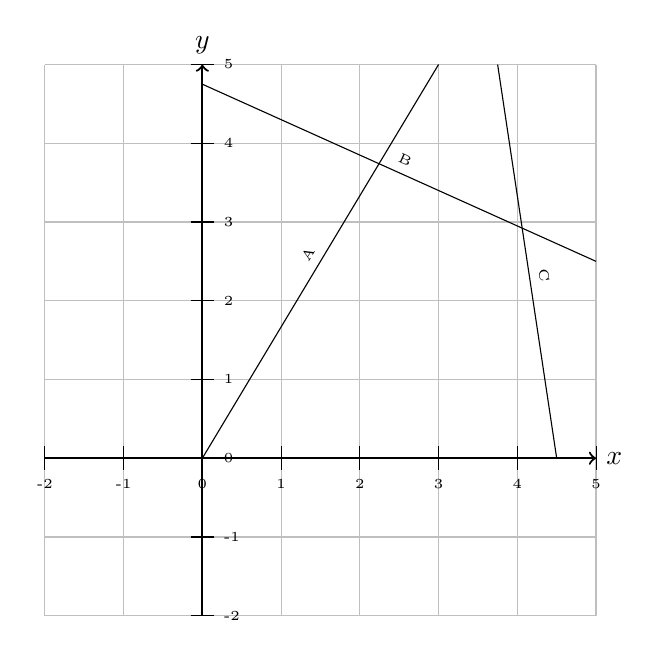
\begin{tikzpicture}
  \draw[gray!50, thin, step=1] (-2,-2) grid (5,5);
  \draw[ thick,->] (-2,0) -- (5,0) node[right] {$x$};
  \draw[ thick,->] (0,-2) -- (0,5) node[above] {$y$};

 \foreach \x in {-2,...,5} \draw (\x,0.15) -- (\x,-0.15) node[below] {\tiny\x};
 \foreach \y in {-2,...,5} \draw (-0.15,\y) -- (0.15,\y) node[right] {\tiny\y};

  \draw (0,0) -- node[above,sloped]       {\tiny A}   (3,5);
  \draw (5,2.5) -- node[above,sloped]       {\tiny B} (0,4.75);
  \draw (4.5,0) -- node[above right,sloped] {\tiny C} (3.75,5);
\end{tikzpicture} 

\begin{parts}
\part On the graph above, draw the convex full that constitutes an ideal formulation.
\end{parts}
\end{center}
		\item We could also ask them why the convex hull is \emph{ideal}?
		\item We could ask them a graph of the LP-relaxation. We could then ask them add constraints that provide a \emph{tighter} formulation but does not provide the convex hull
	\end{itemize}
	\item Branch and Bound
	\begin{itemize}
		\item Here, we could given them a partial B\&B tree and ask them to tell us whether or not each node should be pruned, is active, or incumbent. We could ask them to provide the current upper and lower bounds to the IP.
		\item And, we could ask them to determine the next step in the B\&B algorithm.
	\end{itemize}

\begin{center}
\begin{forest}
  branch and bound,
  where level=1{
    set branch labels={x\leq}{}{x\geq}{},
  }{
    if level=2{
      set branch labels={y \leq }{}{y \geq }{},
    }{},
  }
  [x:{\ Solution, \ z \ }:y]
\end{forest}
\end{center}

\begin{center}
\begin{forest}
  branch and bound,
  where level=1{
    set branch labels={x\leq}{}{x\geq}{},
  }{
    if level=2{
      set branch labels={y \leq }{}{y \geq }{},
    }{},
  }
  [{5.25}:{\ S_0,1055.56 \ }:0.75
    [5:{\ S_1,1000 \ }:5:5
    ]
    [6:{\ S_2, 1033 \ }:1.25:6
      [6.11:{\ S_2,1033 \ }:{1}:1]
      [INF:{\ S_2,inf\ }:inf:2]
    ]
  ]
\end{forest}
\end{center}
\end{itemize}

\begin{parts}
\part What is the current incumbent solution?
\part Clearly label each node as \emph{incumbent}, \emph{active}, or \emph{fathomed}.
\part On which active node should we branch next? Draw the next set of branches on the graph along with the appropriate inequalities.
\end{parts}

\end{document}

\question[10]
Due to an increase in crime rates, Gotham City decides to install special agents at selected restaurants throughout the city.  They would like for every major shopping area to be within 8 minutes of one of these special agents.  City planners develop the following integer program to determine the number of special agents the city will need to hire and train.

Sets and parameters:
\begin{itemize}
\item[] $R = $ the restaurant locations where a special agent could be installed
\item[]
$S = $ the major shopping centers in the city
\item[] 
$t_{r,s} = $ the time to reach shopping center $s$ from restaurant $r$, for $s \in S$ and $r \in R$
\end{itemize}

Variables:
\begin{itemize}
\item[] $x_r = \left\{
\begin{array}{ll}
1 & \text{ if restaurant $r$ is selected as a special agent location } \\
0 & \text{ otherwise }
\end{array}\right.$
for $r \in R$
\end{itemize}

\begin{flalign}
      \text{minimize} \quad & \sum_{r \in R} x_r  \\
      \text{subject to} \quad & \sum_{\underline{~~~?~~~}} x_r \geq 1,~ \forall~  \underline{~~~?~~~} \\ 
                       & x_r \in \{0,1\},~ \forall~ r \in R \nonumber
\end{flalign}

\begin{parts}
	\part Explain the purpose of the constraint labeled (2). 

\answerboxone{c}{1.7in}

\smallskip

	\part Complete the set of constraints labeled (2). Clearly define and explain any additional sets or parameters needed to model these constraints.

\answerboxone{c}{2in}


\vspace{1cm}
\end{parts} 
\newpage
\question[20] (\emph{This is a continuation of question 1.}) Members of the Gotham City budget office determine that the city can afford to staff only 35 special agent locations, and would like to choose the 35 restaurant locations that will maximize the number of shoppers that are within 8 minutes of one of the selected restaurants.  In an effort to update the model to the new problem, city planners collect the following additional data and define the following new variables.
	
Parameters:
\begin{itemize}
\item[] $p_{s} = $ the number of shoppers at shopping center $s$ during peak hours, for $s \in S$
\end{itemize}

Variables:
\begin{itemize}
\item[] $z_s = \left\{
\begin{array}{ll}
1 & \text{ if shopping center $s \in S$ is within 8 minutes of at least one selected restaurant } \\
0 & \text{ otherwise }
\end{array}\right.$
\end{itemize}

Help the planners write the updated model:
\begin{parts}
\part Write the new objective function in \textbf{abstract} form. \vspace{.05mm} \\

\answerboxone{c}{2in}
\vspace{1cm}
\part Write a constraint in \textbf{abstract} form that ensures exactly 35 restaurant locations are selected.\vspace{5mm}\\
\answerboxone{c}{2in}
\vspace{1cm}
\newpage
\part Write a set of constraints in \textbf{abstract} form that enforce the correct behavior of the $z$ variables.\vspace{5mm}\\
\answerboxone{c}{2in}
\vspace{1cm}
\part Explain the purpose of the constraint that you wrote in part (c).\vspace{5mm}\\
\answerboxone{c}{2in}
\end{parts}

\newpage

\question[20] Following a natural disaster, quickly restoring roads in a city is very important to ensure that each house in a neighbor can be reached. Traveling from one house to another may be particularly difficult after hurricanes because the debris and mud can easily cover the entire road. The mayor of the city decided that some of the streets must be clear and restored, but they do not want to spend more money than necessary to ensure they have appropriate funds to use for future hurricane relief. The mayor therefore specified the two following conditions:
\begin{itemize}
    \item [i.] Enough roads must be cleared so that it is possible for everyone to travel from their
house to every other house along clear roads.
    \item [ii.] The restoration process should cost as little as possible.
\end{itemize}

City planners defined the following sets and parameters for an integer program model that will solve the problem.
\begin{itemize}
    \item [] Sets:
	\begin{itemize}
		\item [] $H:=$ Set of houses.
		\item[] $E:=$ Set of roads between houses $i$ and $j$ in $H$.
	\end{itemize}
\vspace{.5cm}
    \item[] Parameters:
    \begin{itemize}
	\item []$c_{ij}:=$ Cost of restoring road $(i,j)$, for all $ \in E$.
    \end{itemize}
\vspace{.5cm}
\end{itemize}

Help city planners complete the integer progam whose solution determines the set of roads to clear first.

\bigskip
\begin{parts}
\item Clearly define any needed variables.

  \medskip
\answerboxone{c}{2in}

\newpage

\item Formulate an \textbf{abstract} integer programming model for solving the mayor's problem. 
\answerboxone{c}{3in}
\vspace{.25cm}
\item Label and briefly explain each constraint.\\
\answerboxone{c}{4in}
\end{parts}





\newpage

\question[20] A metal manufacturer is in the process of designing their new metal sheets. These plates contain 5 different holes that must be drilled by a large drill. The designer's task is thus to determine the order in which each hole is drilled. We assume that the drill must drill each hole, and the drill must return to its initial position after drilling the last hole. The plates are manufactured as mass production, so it is important to determine the minimum time drilling sequence. Our boss has provided the following table that provides the time it takes the drill to move from one position to another (in minutes):
\begin{center}
\begin{tabular}{|c|c|c|c|c|c|}
\hline
Hole \# &  1	&	2	&	3	&	4	& 5\\ \hline
1 & - & 1&2 &3 &6 \\ \hline
2 &- & -& 7& 4& 5\\ \hline
3 &- & -&- & 2 & 8 \\ \hline
4 &- & -& -& -&4 \\ \hline
5 &- &- &- &- &- \\
\hline		
\end{tabular}
\end{center}
\vspace{0.2 cm}

\begin{parts}
    
    \item Formulate the metal manufacturer's task as an integer programming model in the \textbf{concrete} form. Please clearly define all variables, objective function, and constraints. \\
\answerboxone{c}{3in}

    \newpage
\vspace{.5cm}
    Consider the graph below that depicts the metal sheets in the problem above.





\includegraphics[width=\linewidth]{MetalSheetFig.pdf}



 
	\item Run three iterations of the Nearest Neighbor Algorithm originating at holes 1, 3, and 5. Provide the respective sequences that begin at each of these nodes.\vspace{.5cm}
\answerboxone{c}{4in}
    
\end{parts}




\newpage
\question[10] Your regional manager, Michael Scott, has asked you to solve a Vehicle Routing Problem (VRP) to determine an optimal set of 3 paper-delivery routes that begin and end at their warehouse in Scranton, PA. He also tells you that his goal is to minimize the total distance traveled among all vehicles.

\vspace{.5cm}
Answer the following questions related to Michael Scott's request.
\begin{parts}
\item You solve the problem, and your solution contains a cycle of customers that do not contain the warehouse in Scranton. Does this solution provide an upper bound or a lower bound on your optimal vehicle routing solution? Justify your response.\\
\answerboxone{c}{1.5in}
\item Now, Michael Scott tells you that each vehicle can travel no more than $D$ total miles on its route. Is this new problem a restriction or a relaxation to the original problem? Justify your response.\\
\answerboxone{c}{1.5in}
\item Michael Scott also informs you that you are able, but not required, to use 4 vehicles instead of 3. Now, do you expect your optimal solution to this new problem to increase or decrease? Justify your response.\\
\answerboxone{c}{1.5in}
\end{parts}






%\newpage
\question The Superintendent asks his most trusted Ops Research majors (you all) to give him directions from the Yard to Los Angeles, CA. Of course, he wants to find the path the minimizes his total travel time. Assume that he can travel through a set of cities $\mathcal{C}$ along a set of roads $\mathcal{A}$ between each city. He assumes that traveling along some arc $(i,j) \in \mathcal{A}$ will require $t_{ij} > 0$ minutes.  


\begin{parts}

\part Define your starting node $s$ and your destination/termination node $t$. Using these definitions, formulate an abstract mathematical programming model to help the superintendent solve his problem.

%\vspace{11cm}

\part The superintendent now wants to consider traffic delays in each city. To account for this added time it takes to travel through each city, he assumes that it will take $d_i > 0$ extra units of time to travel through city $i \in \mathcal{C}$. Modify your mathematical programming model above to account for the extra traffic-related time delays.
\end{parts}



\question[1] Calculate 2+2.
\addpoints

\question[20] Consider the function $f(x)=3x^3+2x^2+x+1$.
\noaddpoints % to omit double points count
\begin{parts}
\part[10] Calculate $f'(x)$.
\part[10] Calculate $f''(x)$.
\end{parts}
\addpoints

\question[2] One of these things is not like the others; one of these
things is not the same. Which one is different?
\begin{choices}
\choice John
\choice Paul
\choice George
\choice Ringo
\choice Socrates
\end{choices}

\question[2] One of these things is not like the others; one of these
things is not the same. Which one is different?
\begin{oneparchoices}
\choice John
\choice Paul
\choice George
\choice Ringo
\choice Socrates
\end{oneparchoices}

\question[3] Mark box if true.
\addpoints
\begin{checkboxes}
\choice 2+2=4
\choice $\frac{d}{dx} (x^2+1) = 2x+1$
\choice The Moon is made of cheese.
\end{checkboxes}

{%
\checkboxchar{$\Box$} % changing checkbox style locally
\question[3] Mark box if true.
\addpoints
\begin{checkboxes}
\choice 2+2=4
\choice $\frac{d}{dx} (x^2+1) = 2x+1$
\choice The Moon is made of cheese.
\end{checkboxes}
}%

{%
% changing choice items style locally
\renewcommand*\thechoice{\arabic{choice}} 
\renewcommand*\choicelabel{\thechoice)}
%
\question[2] Element with $Z=92$ is:
\begin{multicols}{2}
\begin{choices}
\choice H
\choice O
\choice F
\choice S
\choice Ba
\choice Pb
\choice U
\choice Pu
\end{choices}
\end{multicols}
}%

\question[10]
In no more than one paragraph, explain why the earth is round.
\makeemptybox{2in}

\question[20]
Explain blah, blah\ldots
\makeemptybox{\fill}

\newpage

\question[20]
Explain blah, blah\ldots
\fillwithlines{\fill}

\newpage

\question[20]
Explain blah, blah\ldots
\fillwithdottedlines{8em}







\end{questions}

\end{document}
